%% tags: doubleArrow square leftMargin
\PassOptionsToPackage{usenames,dvipsnames}{xcolor}
\documentclass[tikz,border=2]{standalone}
\usepackage{amssymb}
\usepackage{enumitem}
\usepackage{mathtools} % contains amsmath which comes with align
\usepackage{amsthm}
\usepackage{graphicx}
\usepackage{microtype} % some compression
\usepackage[skins]{tcolorbox}
%%%%%%%%%%
%% \definecolor{LightBlue}{HTML}{38BFB3}
%% \definecolor{DarkBlue}{HTML}{3E6A74}
%% \definecolor{LightGreen}{HTML}{99DB3B}
%% \definecolor{Orange}{HTML}{F4AD2F}
%% \definecolor{Red}{HTML}{F56544}
%% \definecolor{Pink}{HTML}{EF386D}
%%%%%%%%%%
% brown blue red
\definecolor{LightBlue}{HTML}{C7DFE3}
\definecolor{DarkBlue}{HTML}{72AFB6}
\definecolor{DarkBrown}{HTML}{D2BE89}
\definecolor{LightBrown}{HTML}{F4ECDF}
\definecolor{Grey}{HTML}{A7A195}
\definecolor{Red}{HTML}{CA6C2E}
%%
\def\labelitemi{\textcolor{gray}{\tiny{$\blacksquare$}}}
%%
\usetikzlibrary{shadows,arrows,shapes,positioning,calc,backgrounds,
fit,automata,decorations.markings,
decorations.pathreplacing,decorations.pathmorphing}
%%%%%%%%%%%%%%%%%%%%%%%
\begin{document}
\begin{tikzpicture}
[scale=1,auto, transform shape,
show background rectangle,
background rectangle/.style={fill=white},
every node/.style={align=left},
titleblock/.style={font=\large,font=\bf,rectangle,minimum width=1cm,text=white,fill=black!50},
descblock/.style={font=\small,black!80,draw=black,thick,rectangle,minimum width=2cm},
anc/.style={shape=circle,inner sep=3pt,fill=black},
vecArrow/.style={thick, decoration={markings,mark=at position 1 with
{\arrow[semithick]{open triangle 60}}}, double distance=3.5pt, shorten
>= 6.5pt, preaction = {decorate}, postaction = {draw,line width=1.4pt,
white,shorten >= 5.5pt}},
cedge/.style={draw=black,>=latex', shorten >=.0pt, shorten <=.0pt, 
thick},
tedge/.style={draw=black,>=latex', shorten >=.0pt, shorten <=.0pt, 
semithick},
iedge/.style={draw=black,>=latex', shorten >=.0pt, shorten <=.0pt, ultra
thick, dashed}]
%%%%%%%%%%%%%%%%%%%%%%%%%%%%%%%%%%%%%%%%%%%%%%%%%%%%%%%%%%%%%%%%%%%%%%%%%%%
%% Digital library
%%%%%%%%%%%%%%%%%%%%%%%%%%%%%%%%%%%%%%%%%%%%%%%%%%%%%%%%%%%%%%%%%%%%%%%%%%%
\node (dlDesc) [descblock,minimum width=4.5cm,draw=DarkBlue,shift={(0,-.5)}]{\parbox{4.3cm}{
%%\colorbox{DarkBlue}{\textcolor{white}{Digital library}}
{\textcolor{DarkBlue!180}{Digital library}}
\vspace{.2cm}
\begin{itemize}[leftmargin=*]
\item Data integration and linking
\item Metadata and semantic mapping
\item Data quality and accuracy
\item Querying, analytics, and APIs
\end{itemize}}};
%%
\node (dlTitle) [fill=white,above left=-.7cm and -4.9cm of
dlDesc]{
\includegraphics[width=1cm]{aux/library_DarkBlue.png}};
%%
%% \node (dlTitle) [titleblock,fill=DarkBlue,text=white,align=left,above left=-.4cm and -2.3cm of
%% dlDesc,]{Digital library};
%%%%%%%%%%%%%%%%%%%%%%%%%%%%%%%%%%%%%%%%%%%%%%%%%%%%%%%%%%%%%%%%%%%%%%%%%%%
%% Synthetic population 
%%%%%%%%%%%%%%%%%%%%%%%%%%%%%%%%%%%%%%%%%%%%%%%%%%%%%%%%%%%%%%%%%%%%%%%%%%%
\node (gp) [descblock,draw=DarkBlue,left=2cm of dlDesc]{\parbox{3.5cm}{
%%\colorbox{DarkBlue}{\textcolor{white}{Synthetic Population}}
{\textcolor{DarkBlue!180}{Synthetic Population}}
\vspace{.2cm}
\begin{itemize}[leftmargin=*]
\item synthetic networks
\item $3$ West African countries
\end{itemize}}};
%%
%%%%%%%%%%%%%%%%%%%%%%%%%%%%%%%%%%%%%%%%%%%%%%%%%%%%%%%%%%%%%%%%%%%%%%%%%%%
%% BSVE-API
%%%%%%%%%%%%%%%%%%%%%%%%%%%%%%%%%%%%%%%%%%%%%%%%%%%%%%%%%%%%%%%%%%%%%%%%%%%
\node (bsveAPIDesc) [descblock,draw=DarkBlue,above=1.5cm of dlDesc]{\parbox{3.9cm}{
%%\colorbox{DarkBlue}{\textcolor{white}{BSVE APIs \& tools}}
{\textcolor{DarkBlue!180}{BSVE APIs \& tools}}
\vspace{.2cm}
\begin{itemize}[leftmargin=*]
\item Middleware
\item BSVE SDK
\end{itemize}}};
%%
\node (bsveAPITitle) [fill=white,above left=-.9cm and -4.4cm of
bsveAPIDesc]{
\includegraphics[width=1cm,angle=-90]{aux/services_DarkBlue.png}};
%%%%%%%%%%%%%%%%%%%%%%%%%%%%%%%%%%%%%%%%%%%%%%%%%%%%%%%%%%%%%%%%%%%%%%%%%%%
%% World map
%%%%%%%%%%%%%%%%%%%%%%%%%%%%%%%%%%%%%%%%%%%%%%%%%%%%%%%%%%%%%%%%%%%%%%%%%%%
\node (globe) [above left=-.5cm and 1cm of
dlDesc]{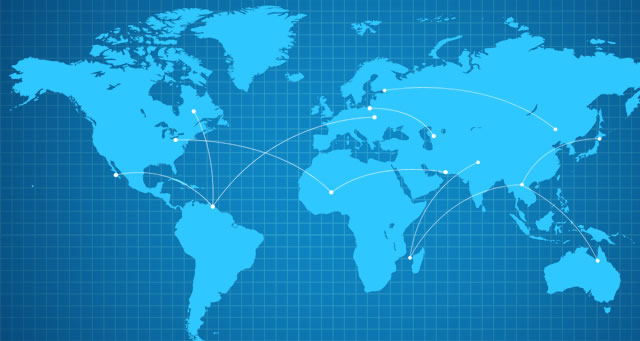
\includegraphics[width=7cm]{aux/world_map.png}};
%% %%%%%%%%%%%%%%%%%%%%%%%%%%%%%%%%%%%%%%%%%%%%%%%%%%%%%%%%%%%%%%%%%%%%%%%%%%%
%% %% Survey
%% %%%%%%%%%%%%%%%%%%%%%%%%%%%%%%%%%%%%%%%%%%%%%%%%%%%%%%%%%%%%%%%%%%%%%%%%%%%
%% \node (surveyDesc) [descblock,draw=LightBlue,above =.5cm of
%% globe]{\parbox{4.5cm}{
%% \begin{itemize}
%% \item Mobility \& behavioral data
%% \item WiSDM
%% \item ground connectivity
%% \item eliciting expert judgement
%% \vspace{.5cm}
%% \end{itemize}}};
%% %%
%% \node (surveyTitle) [titleblock,below right=-.4cm and -1.9cm of
%% surveyDesc,fill=LightBlue]{Survey data};
%%%%%%%%%%%%%%%%%%%%%%%%%%%%%%%%%%%%%%%%%%%%%%%%%%%%%%%%%%%%%%%%%%%%%%%%%%%
%% DDL
%%%%%%%%%%%%%%%%%%%%%%%%%%%%%%%%%%%%%%%%%%%%%%%%%%%%%%%%%%%%%%%%%%%%%%%%%%%
\node (ddlDesc) [descblock,draw=Red,above=1.25cm of globe,shift={(0,0)}]{\parbox{4.6cm}{
%%\vspace{.5cm}
   %% \colorbox{Red}{\textcolor{white}{Data from USAID projects}}
   {\textcolor{Red!122}{Data from USAID projects}}
\vspace{.2cm}
\begin{itemize}[leftmargin=*]
\item Development Data Library (DDL)
\item DHS program
\end{itemize}}};
%%
\node (ddlTitle) [fill=white,above left=-.7cm and -5.2cm of
ddlDesc]{
\includegraphics[width=1cm]{aux/database_Red.png}};
\node (usaidArr) [double arrow,Red,draw,minimum height=1.2cm,thick,right =.15 of ddlDesc] {};
%%%%%%%%%%%%%%%%%%%%%%%%%%%%%%%%%%%%%%%%%%%%%%%%%%%%%%%%%%%%%%%%%%%%%%%%%%%
%% DDL-API
%%%%%%%%%%%%%%%%%%%%%%%%%%%%%%%%%%%%%%%%%%%%%%%%%%%%%%%%%%%%%%%%%%%%%%%%%%%
\node (ddlAPIDesc) [descblock,draw=Red,right=1mm of usaidArr]{\parbox{3.9cm}{
   %%\colorbox{Red}{\textcolor{white}{Existing APIs \& tools}}
   {\textcolor{Red!122}{Existing APIs \& tools}}
\vspace{.2cm}
\begin{itemize}[leftmargin=*]
\item DHS program API
\item DHS statcompiler
\end{itemize}}};
%%
\node (ddlAPITitle) [fill=white,above left=-.9cm and -4.4cm of
ddlAPIDesc]{
\includegraphics[width=1cm,angle=-90]{aux/services_Red.png}};
\node (bsveArr) [double arrow,DarkBlue,draw,rotate=90,minimum
height=1.2cm,thick,above=.7cm of dlDesc] {};
%%%%%%%%%%%%%%%%%%%%%%%%%%%%%%%%%%%%%%%%%%%%%%%%%%%%%%%%%%%%%%%%%%%%%%%%%%%
%% End user
%%%%%%%%%%%%%%%%%%%%%%%%%%%%%%%%%%%%%%%%%%%%%%%%%%%%%%%%%%%%%%%%%%%%%%%%%%%
\node (euTitle) [right=of
bsveAPIDesc,shift={(.5,0)}]{
\includegraphics[width=1cm]{aux/user_DarkBrown.png}};
\node (euDesc) [below=of euTitle,shift={(0,1)}]{\parbox{2.5cm}{
   \colorbox{DarkBrown}{\textcolor{white}{End user}}
   \begin{itemize}[leftmargin=*]
\item domain experts
\item policy makers
\item modelers 
\vspace{.5cm}
\end{itemize}}};
\node (userArr) [double arrow,black!60,minimum height=1.2cm,draw,thick,right=3mm of bsveAPIDesc] {};
%%%%%%%%%%%%%%%%%%%%%%%%%%%%%%%%%%%%%%%%%%%%%%%%%%%%%%%%%%%%%%%%%%%%%%%%%%%
%% globe anchors
%%%%%%%%%%%%%%%%%%%%%%%%%%%%%%%%%%%%%%%%%%%%%%%%%%%%%%%%%%%%%%%%%%%%%%%%%%%
\node (senegal) [anc,DarkBlue,shift={(-.4cm,0.1)}] at (globe) {};
%% \draw[tedge,LightBlue] (senegal) -- ++(0,2) -| ($(surveyDesc.south west)+(1,0)$);
%%
%% \draw[tedge,LightBlue] (tanzania) -- (surveyTitle.south-|tanzania);
%%
\node (southamerica) [anc,Red,left=of senegal,shift={(.2,-.8)}]{};
\draw[tedge,Red] (southamerica) -- ++(0,1.5) -| ($(ddlDesc.south)+(-1,0)$);
%%
\node (africa) [anc,Red,right=of senegal,shift={(-.5,-.2)}]{};
\draw[tedge,Red] (africa) -- ++(0,1.5) -| ($(ddlDesc.south)+(-.25,0)$);
%%
\node (asia) [anc,Red,right=of senegal,shift={(1.1,.3)}]{};
\draw[tedge,Red] (asia) -- ++(0,1.5) -| ($(ddlDesc.south)+(0.75,0)$);
\draw[tedge,DarkBlue] (senegal) -- ($(gp.north-|senegal)$);
%%%%%%%%%%%%%%%%%%%%%%%%%%%%%%%%%%%%%%%%%%%%%%%%%%%%%%%%%%%%%%%%%%%%%%%%%%%
%% arrows
%%%%%%%%%%%%%%%%%%%%%%%%%%%%%%%%%%%%%%%%%%%%%%%%%%%%%%%%%%%%%%%%%%%%%%%%%%%
\draw[iedge,black!60,->] ($(ddlDesc.south east)+(-1,0)$) -- ++(0,-1)
node[anchor=north west,shift={(0,.5)},black]
{Data ingestion} --
++(2.5,0) |- ($(dlDesc.west)+(0,.6)$);
\draw[iedge,black!60,<->] (ddlAPIDesc) -- node [text=black] {Linking apps}
(ddlAPIDesc|-bsveAPIDesc.north);
\draw[iedge,black!60,<->] (dlDesc) -- node [shift={(.2cm,0)},text=black,text width=2cm] {Fusing various datasets}
(gp);
\end{tikzpicture}
\end{document}
